%%%%%%%%%%%%%%%%%%%%%%%%%%%%%%%%%%%%%%%%%%%%%%%
%\chapter{Scaffolding Citizen-led Complex Knowledge Work}
\chapter{Social Computing for Complex Knowledge Work}

\begin{quote}
\emph{This dissertation explores how the following things happen. Complex work is hard. Needs learning. People do things in groups. Social computing misses learning (learning is around but not here). why your title is what it is, what that means, how you set up your arguments, and what claims your introductory chapter makes. Current online platforms (like Facebook) are built on insights from psychology about capturing people’s attention. My research instead takes a more socially responsible approach by integrating learning theory and collaboration for people to perform complex work such as generating and evaluating scientific theories. This has the potential to diversify the stakeholders and contributors to our future society.}
\end{quote}
\vspace{0.25in}

Social computing platforms have revolutionized how most people connect, communicate, and share. We increasingly connect with friends and strangers in different ways for a number of purposes. Friends and family can stay in constant touch with their loved ones. Strangers from different parts of the world discuss their ideas about their health. Increasingly, these connection opportunities have also translated to more active doing: people fund other's\'  ideas that traditional business places might balk at. Some have used social platforms to amplify their voice and bring about social changes. for instance, people in Sudan have taken down dictators [??]. By transforming how we communicate, share, and chat, social computing has become perhaps the greatest internet-fueled change of our times. 

%%interactive vis (social computing discussions) is awesome
% people can do stuff with hypotheses (test them?)
%    however, viz is hard (scientific work)
%        programming toolkits needed and impose burden (support needed to get started, reduce burden, and …)

However, the benefits of social computing are not distributed equally. While everyone has a voice, some have bigger loudspeakers than others: xx\% of most popular posts are from experts. While anyone can organize and bring changes, collective attempts to organize frequently fail. While anyone can learn from widely accessible research papers and articles, people create faulty insights from self-tracking and conspiracy theories abound. With this lens, social computing seems less transformative but rather a highly scaled up version of the offline reality of limited expertise people live in. 
% 1 to 1 link with the first para

%\subsection{Pivot to people - People can do great things but need help...}
%Well, what are people good at? What are they motivated to do? 

%People have complementary knowledge in comparison to experts and are uninfected by expert biases; these insights are drawn from lived experience, both individual and collective.

Specific to this dissertation: While social computing platforms have vastly succeeded at keeping people engaged and sharing, they barely support \textit {citizen-led enquiry}. People have strong personal motivations and contextual insights. People possess a remarkable ability to identify patterns and create theories from their experiences [??]. While most people have an amazing breadth and depth of ideas, they lack the expertise to implement these ideas. To create knowledge, they need mental scaffolds for organizing complex work, domain knowledge to compose and execute the steps, and ways to ask for help. Experts benefit from conceptual knowledge, professional training, pre-existing organizational structure for collaboration, and direct access to resources. Currently, citizens lack these resources. social computing platforms where people spend ridiculous times provide little support. 

%this is the current state --  this is the big challenge, why is it a challenge
%% however, scaling good teaching is hard - kulkarni
%     this peer thing can be helpful (evidence from small studies)
%        however, this is challenging — 2 causes
%        interfaces need to provide scaffolding 


\begin{figure}[b] 
  \centering
  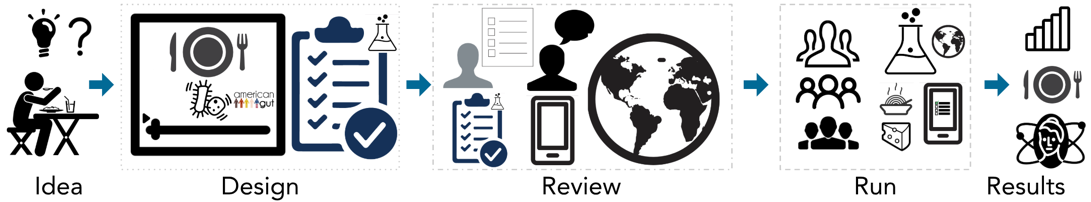
\includegraphics[width=1.0\textwidth]{figures/intro/intro-1}
  \caption[]
{The Gut Instinct platform enables anyone to transform their intuitions to hypotheses 
and then design and run experiments to test them [xx-xx]. Gut Instinct integrates 
conceptual learning embedded via short lectures and software-guided procedural 
learning to enable designing and reviewing experiments. Participants from around
 the world join experiments, follow instructions, and pro-vide data in response to 
automated data collection reminders. }
  \label{fig:intro-1}
\end{figure}

Consequently, this is unfortunate missed opportunity for both individuals and the world at large. Enabling peoplt to learn to perform personally meanignful work can help them answer their own questions. People's ideas can catalyze creating new knowledge that we are missing out on.  How might online systems support citizen-led knowledge work? 

Let''s reflect on this dual nature:  science can answer life-relevant questions but few know how to even get started. As a result, people fail to answer their questions and institutional science misses out on ideas from beyond the ivory tower. 

%one line to summarize my work -- see other intro

%two properties of classes help us - kulkarni
%this thesis leverages these two properties and provides a new class of benefits etc... 

%what helps us
%1. the scientific method is structured
%    1. even though creative and open-ended
%2. roles: people take them online
%    1. captures diversity — breadth
%    2. micro-expertise supports this explicitly 
%3. procedural learning: can teach people how to do things
%    1. captures learning — depth


This dissertation advances the design of social computing systems by integrating learning and collaboration to enable complex work such as generating and evaluating scientific theories. Over 600 people from 30 countries have self-organized to generate theories about the human microbiome and test them by running experiments. This dissertation raises the question: how can global communities create knowledge that meets their goals without waiting for experts to lead? 

Gut Instinct emodies this insight and introduces a collaborative citizen science platform for people to transform lived exes into scientific theories. 

%%%%%%%%%%%%%%%%%%%%%%%%%%%%%%
\section {People already do great things but struggle with complex tasks}

\subsection{People are awesome}
People design, build, and track to better understand and improve their health [?? dana lewis].  On numerous online fora, people share their intuitions, observations, folk theories, and even results from trying different approaches to improve their health, e.g. from simple ideas like ‘giving up drinking coffee to improve quality of sleep’ to tests and dietary approaches. People draw ideas from current research by reading and discussing papers. In many cases, these discussions are not just anecdotal but also derive from state-of-the-art scientific work. In some cases, people contribute back to scientific work as well.How can social computing platforms effectively enable people to do more personally meaningful work built upon their experiences and insights?

People’s curiosity, needs, and possibilities to do useful work is endless; however, traditional online systems don’t support them. Online fora encourage long, rambling discussions. Online learning provides conceptual lessons but people drop out and these are not linked to people’s needs.While learning resources like MOOCs abound, they hardly meet the need: many drop out, the lectures focus on conceptual knowledge, and lack the feedback needed to perform open-ended creative work. We know little about integrating learning resources and social computing affordances are far from each other. Moreover, currently both learning and work are not personal; can we change this? Lack of appropriate "learning abstractions" make complex work unrealistic.

The goal is to create environments for learning and collaboration through complex, personally meaningful work.

%%%%%%%%%%%%%%%%%%%%%%%%%%%%%%%%%%%%%%%%%%%%%%%%%%%
\subsection{Challenge: People' don't know what to do and how to do it}
Citizens have a different background than professional scientists; they have unique
 personal experiences but lack the years of domain training. Two major issues in 
enabling complex work on the internet are (diversity and scale?) 
quality of individual contribution and managing overall contributions from the crowd.
We desire social computing techniques that reliably enable a wide variety of people to 
contribute more than they naturally could and that manage the dependencies among
 a large set of tasks.

To create computational systems that leverage their strengths and mitigate the lack of training, this dissertation 
focuses on domains where the science is nascent, highly contextual, and personally motivating.
 Synthesizing the crowdsourcing literature and my experience highlights three challenges: 
poor signal-to-noise from crowds due to lack of training; inefficient collaboration without 
careful attention; and poor results (or no results at all) unless experts lead. 

To address  these concerns,  this dissertation introduces and evaluates peer production architectures 
and procedural learning.

\subsection{Scientific experimentation: An instance of complex knowledge work}
%here''s an example: experimentation 
Supporting complex knowledge work has been a challenge for Human Computer Interaction
 research (make specific). For instance, many people are interested in understanding and 
improving their health. Millions of peple from all over the world share their insights. 
Can't they run experiments for these?

Scientific experimentation features technical requirements and contextual choices 
that are inscrutable for a lay individual yet necessary for success [??]. While 
professional scientists and commercial ventures run experiments every day, with 
notable exceptions [??], empirical papers from non-professionals are 
vanishingly rare. This biases the questions asked, studies run, and knowledge 
created [??]. People have questions about their health, but lack the expertise 
and resources to scientifically investigate them. Broadening the pool of 
experimenters could help people investigate their curiosities, develop solutions 
to improve health and performance, and assist institutional researchers.


\textit{People lack the expertise to know what to do and how to do it.}. 
Success with complex creative activities requires procedural
knowledge (how to do things) in addition to conceptual
knowledge (facts). While many resources offer facts, procedural
learning is often ignored.The converse also holds, and much more often: novices are also
“uninfected” by all the knowledge that enables experts to
innovate.Sometimes, having a different background than experts can
be beneficial. Shared knowledge is great when it’s right, but
blocks progress when wrong. When false assumptions limit
experts, at least some novices are likely to be “uninfected”.
For example, GalaxyZoo volunteers discovered ‘green pea’
galaxies overlooked by scientists who mistakenly assumed
the green hue was merely an imaging artifact [54]. 


% kulkarni -- "This assessment requires bothcommon-sense knowledge to understand student work and the expertise to assess tacit criteria such as “well-designed” or “well-modularized” that cannot be completely articulated. Indeed, teaching such tacit criteria is an important goal in open-ended domains like design"


\textit{People lack a professional network to improve their work}. 
Furthermore,  how do people ask others for help? Who do they reach out to?

People are connected online and collectively have access to many resources.
In a large distributed community, there’s often someone who happens to 
have important relevant knowledge, usually drawing on a relevant but 
distant domain. Such distributed efforts are a type of lead-user innovation [31]. 
Having many people work on the same problem increases the odds that 
one will break through. Drawing on secondary expertise as inspiration can
 be an important agent of creativity because almost by definition, the 
combination is rare [10]. %Open \& crowd innovation builds up on contributions
 by diverse online participants, and a ‘bubbling up’ process for strong ideas [56].

While many hands make light work, novices need clear contribution opportunities. 
The crowdsourcing literature offers many good verification approaches for tasks 
with clear right or wrong answers – like whether two images represent the same 
product or what street number is written on a sign. However, verifying knowledge
 work necessitates a different approach because it requires making 
situationally-appropriate choices. 

%%%%%%%%%%%%%%%%%%%%%%%%%%%%%%%%%%%%%%%%%%%%%%%
\section{Thesis Statement and Contributions}
\noindent This dissertation investigates the question: how to enable people to perform personally meaningful work otherwise beyond their expertise? Underlying these investigations is the thesis:
%"My thesis statement is"
\begin{quote}
\emph{Providing task-specific guidance in social computing enables personally meaningful \& useful scientific work}
\end{quote}

This dissertation\textquotesingle s primary contribution is the idea of intergrating learning in social computing to enable groups of novices to perform complex, creative activities. The thesis achieves this integration by building a sequence of interactive prototypes that enable people to collaboratively generate and test hypotheses. In the process, the prototypes divide complex work into distinct activities: self-sourcing the design and crowdsourcing people''s inputs and data. Every prototype advances social computing further as a domain for deep, personally meaningful work. Beyond introducing learning abstractions, this dissertation carefully designs the affordances, support, and system to enable different users for different needs. 

 %To realize this idea, 
This dissertation makes three types of contributions: theoretical perspectives/techniques, real-world systems, and outcomes including empirical results, systems lessons, and dataset (Figure \ref{fig:contributions}). 

%%%%%%%%%
\subsection{Theoretical  Techniques}
Improving  work quality in social computing suggests deepening individual contributions and broadening participation by providing different contribution mechanisms.The former requires better learning tools and the latter requires better collaboration tools and dependency management. Consequently, this thesis' theoretical contributions include 1) principles to integrate guidance for complex tasks, and 2) ways to divide complex tasks into multiple roles or affordances.

%“..adapts and extends techniques from xxx” -  arvind

%system-led learning vs people-led
Traditional systems think of knowledge as being provided by the people, while we being the knowledge from the system itself.

%todo-introduce the learning and collaboraiton taxonomy here
\begin{figure}[b] 
  \centering
%  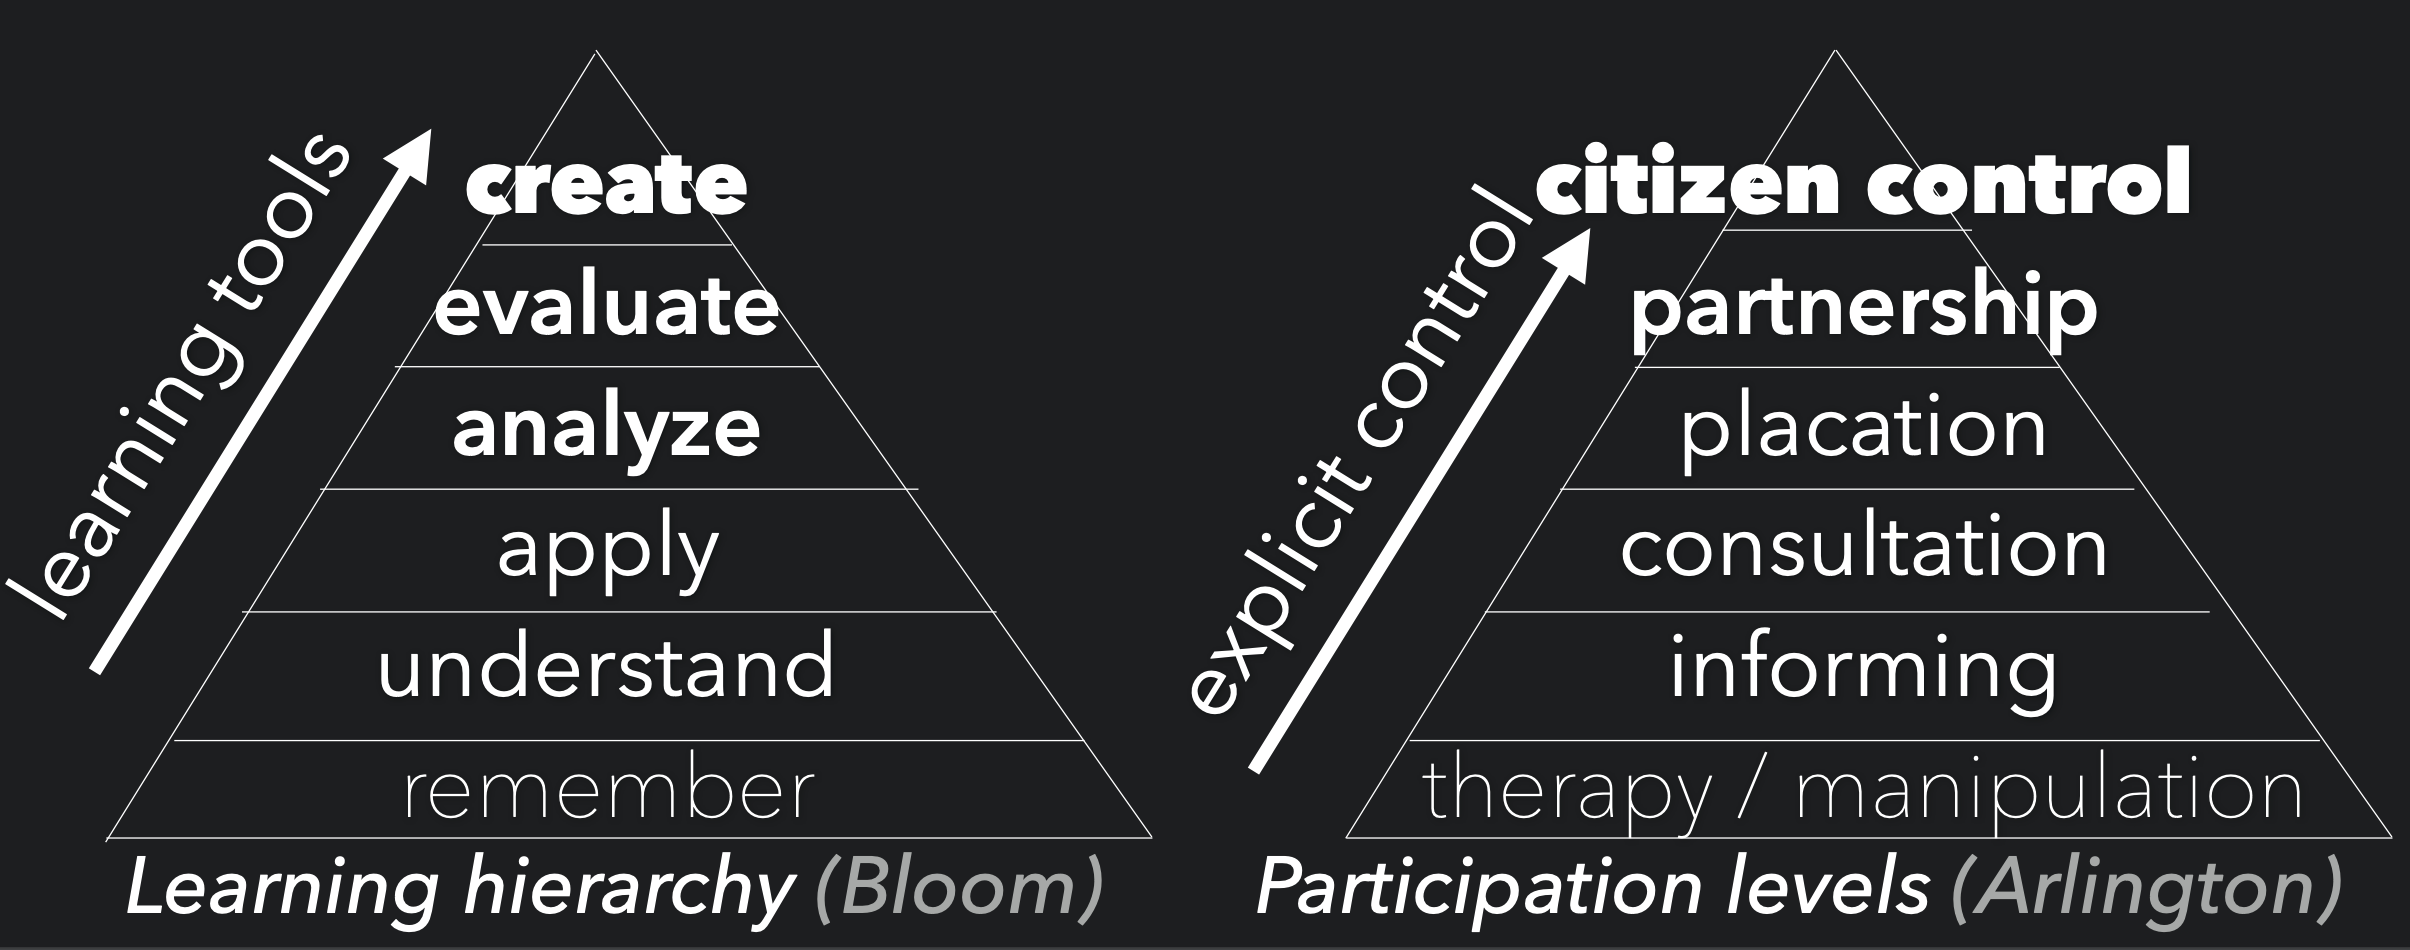
\includegraphics[width=1.0\textwidth]{figures/intro/intro-taxonomy}
  \caption[]
{Drawing from Maslow's hierarchy of learning and xx's hierarchy of contribution}
  \label{fig:intro-taxonomy}
\end{figure}

% come up with principles myself
%figure about conceptual and procedural learning 
\textit{Principles to integrate learning in social computing}: Learning broadly comprises conceptual (declarative) and procedural knowledge. Conceptual learning is where people learn what something is, learn about its features; this is a big part of current teaching. Typically, such learning is tested with test questions. In contrast, procedural learning teaches the {\it how} of things. How do you do x, y, or z.  Concpetual learning is useful when xxx while procedural learning is more useful when yyy.

To make useful contribution, people need to have a good working model of both the concepts and procedures for an activity. This dissertation enables this in two ways: 1) reifying conceptual bits in the software, and 2) providing procedural guidance with examples, checklists, and templates. Building on Maslow''s hierarchy~\ref{??}, it aims to push learning more up.

\textit{Principles to decompose Complex work to f(people, community, \& machines)}
% figure -- def needs one -- based on strengths and weaknesses
%fig - present a stack of things
The individual, groups of people, and machines possess complementary strengths. Individuals have personal motivation to do something; their lived experiences provide ideas that might be potentially novel. Groups of people might not be as motivated but might be willing to help by providing another set of eyes and complementary knowhow and insights from lived expeirences; they can help check biases with the diversity of their lived experiences. But since they are not as motivated, maybe limited affordances would be useful. Computers can implement things consistently to reduce biases but they cannot interpret open-ended instructions fairly in different contexts the way people can.  (todo- fix this to crisp english writing) (see slide deck)

Given these complementary strengths and limitations, this dissertation 1) begins every task with a heavy-handed implementation by an individual personally invested in that idea, 2) improves it with others'' feedback, and finally, 3) runs the idea with the help of automated software. For all these steps, the system manages the interdependencies beneath the sheets to reduce pressure on people. Building on xx's hierarchy~\ref{??}, it aims to push collaboration more up.

The efficacy of these techniques is borne out over multiple deployments. All these techniques have been put in systems as interfaces, intelligent backends, and so on... \\

%\begin{figure}[t!] 
%  \centering
%    \includegraphics[width=1.0\textwidth]{figures/img/intro/1-contributions}
%  \caption[Contributions of this dissertation]
%{Contributions of this dissertation including empirical results theoretical perspectives/techniques, real-world systems, and multiple outcomes}
%  \label{fig:contributions}
%\end{figure}

\subsection{User Interface and System Design}
%User interfaces and system design for efficient implementation
%figs needed to explicate 

While guidance techniques and role differentiation provide the building blocks, they are by themselves insufficient for useful higher-order collaborative work. These techniques need to be baked in simple, interactive interfaces. Multiple challenges show up for this question. First, the internet is a diverse community and have varying levels of expertise. So, the things need to be understandable to all. Second, people might have poor models of thiking about stuff and might frame their ideas and intuitions in weird ways.Third, the interface should make it easy to keep moving and get unstuck.  Too much information might make people struggle, so we need UIs for focused collaboration. 

This dissertation by bakes the techniques in the user interface  and by building a backend that is based on the principles of x, y, and z.

%System contributions
Gut Instinct  introduces a collaborative citizen science platform for people to transform lived exes into scientific theories. Gut Instinct frames the task of hypothesis-testing as a crowdsourcing problem, develops techniques and platform that supports different roles with just-in-time learning, and provides efficient backend support to automate simple tasks.

Gut Instinct divides multi-party collaboration into complementary tasks and supports them using different contribution mechanisms (like adding a question, editing a response) and roles (like experimenter, reviewer, participant). This provides people the flexibility to choose how much they’d like to contribute. Finally, Gut Instinct automatically manages multiple activities to reduce 
bias and experimenter/participant workload,such as randomized placement of 
people into conditions, maintaining anonymity, and collecting and cleaning data.


Take for instance, the state diagram — the edges represent what people need to do 
Roles Support via Just-in-time Skill Acquisition:  People take different roles--write up form galileo

%%"Furthermore, adding location information to photo collections is by itself insufficient for scenevisualization: we also need intuitive, interactive interfaces for exploring these scenes. There are several challenges faced in the design of such interfaces. First, unlike with Google Street View, where photos are taken at regular intervals, personal or Internet collections are typically an unstructured soup of photos. Nevertheless, the navigation controls should still be intuitive and exhibit regularity. Second, such controls should make it easy to find and explore the interesting parts of a scene, particularly for tourist sites."

%%%%%%%%%%%%%
\subsection{Outcomes}
\subsubsection{Empirical Results from Real-world Deployment}
expertise: limited; diversity: different countries; scale: some

\subsubsection{Dataset}
1. repo of hypotheses with rating
2. repo of experimental designs
3. ...

\subsubsection{Impact}
344 volunteers from 27 countries created 399 hypotheses about their health and the gut microbiome. Remarkably, microbiome scientists rated a fifth (75) of these hypotheses to have a scientifically valuable insight about a topic not covered by existing published work. Volunteers fleshed out 60 of these hypotheses into complete experimental designs. My entire work (code + data) is open source so others can edit, build, and experiment.

This dissertation has also enjoyed sufficient support in multiple research communities: Innovation researchers at MIT, online and offline fermentation and self-tracking communities, and citizen science groups. Finally, parts of the system have been taught in classrooms including CSCI 499: (Computing for Social Good) at USC. 

This work explores how online learning and process training systems, combined with
peer collaboration, can help people learn similar skills that
can be useful in scientific and design domains.


%%%%%%%%%%%%%%%%%%%%%%%%%%%%%%%%%%%%%%%%%%%
\section{Dissertation Roadmap}

%%%%%%%%%%%%%%%%%%%%%%%%%%%%%%%%%%%%%%%%%%%%%%%%%%%%%%%%%%%%%%%%%%
%todo- “we” refers to the set of authors…  -- see arvind

My dissertation demonstrates how we might draw on people’s diverse background knowledge, interest, and micro-expertise to expand scientific knowledge and push it in new directions. More specifically, the Gut Instinct platform that I have built instantiates these ideas enabling participants of the American Gut Project (the world’s largest crowdfunded citizen science project) to generate and experimentally investigate hypotheses (Figure 1). 

This dissertation creates the opportunity of harnessing humanity\textquotesingle s collective efforts to accomplish great goals.
s


"double quotes"


%The techniques make the idea concrete; the system operationalizes the techniques and makes them work; and the outcomes discuss the successes and failures of our approach.

%to people for them to perform personally meaningful work.
%My research prototypes collective systems for large-scale problems.
%Worldwide, people use online health fora to share insights and look for answers
%Iin short, to push people towards actively testing their ideas rather than just sharing them?  whether drinking kombucha really changes the gut constitution? In the absence of support and guidance, how can people do more? . 

%%1. novice-led
%    1. no experts
%    2. with other novices 
%2. personally meaningful 
%3. techniques
%    1. expert work to social computing 
%        1. ways to do that
%4. output
%    1. create new knowledge 
